\subsection{Order of Deployment}

Best explained with an example
\href{https://www.warzone.com/MultiPlayer?GameID=36719132}{Chris vs Ragnar, MTL}
I received my first 3 picks. End of turn 3 I meet up an opponent an a very suspicious place. Look at the game from my POV turn 4, specifically the deployments that took place.

\begin{wrapfigure}{r}{0.35\textwidth}
    \centering
    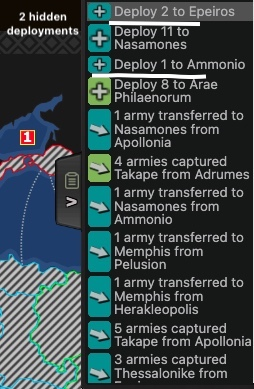
\includegraphics[width=0.25\textwidth]{Images/order_deployments.jpg}
    \caption{History from my POV}
    \label{order_deployments}
\end{wrapfigure}

I deploy 3 times and then I see my opponent's deployment of 8 armies. I can derive from his capture of 4 armies that on that specific turn, I had 1st move. Deployments also follow move order. That means Ragnar deployed in 2 places or more before deploying on the border vs me. Get into the habit of hiding your position and income. If your opponent is repeatedly making this again and again and again, use that information against them.
\\
Another example is \href{https://www.warzone.com/MultiPlayer?GameID=36233122}{Chris vs Gincompetent, 1vs1 Ladder}, Turn 4. I know from the attacks that have taken place, that I have first move on turn 4. And my opponent deploys elsewhere twice, then on me. + I see all his delays. After such a turn you should be able to understand exactly where you opponent is. Invest those 3 minutes to understand the position and find the winning moves.